\begin{figure}
  \centering
  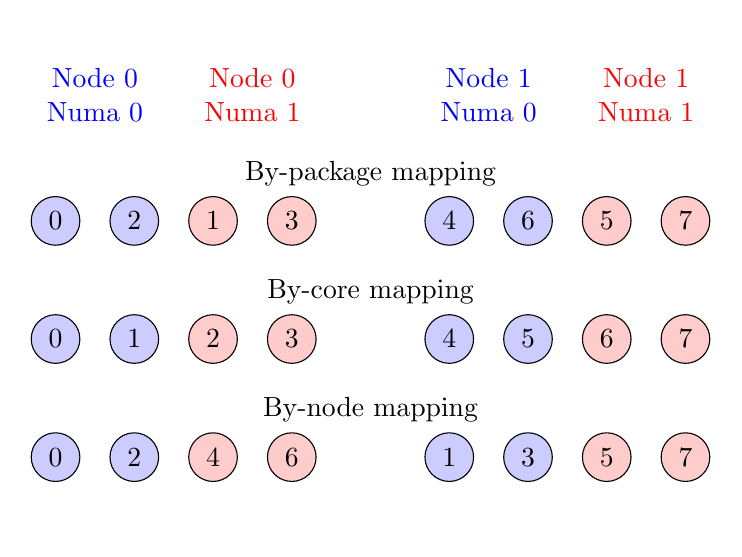
\begin{tikzpicture}[every node/.style = {shape=circle, draw, align=center}]
    \node at (0.5, 4.6) [draw=none, text=blue] {Node 0\\Numa 0};
    \node at (2.5, 4.6) [draw=none, text=red] {Node 0\\Numa 1};
    \node at (5.5, 4.6) [draw=none, text=blue] {Node 1\\Numa 0};
    \node at (7.5, 4.6) [draw=none, text=red] {Node 1\\Numa 1};
  
    \node at (0, 3) [fill=blue!20] {0};
    \node at (1, 3) [fill=blue!20] {2};
    \node at (2, 3) [fill=red!20] {1};
    \node at (3, 3) [fill=red!20] {3};
    \node at (4, 3.6) [draw=none] {By-package mapping};
    \node at (5, 3) [fill=blue!20] {4};
    \node at (6, 3) [fill=blue!20] {6};
    \node at (7, 3) [fill=red!20] {5};
    \node at (8, 3) [fill=red!20] {7};
    
    \node at (0, 1.5) [fill=blue!20] {0};
    \node at (1, 1.5) [fill=blue!20] {1};
    \node at (2, 1.5) [fill=red!20] {2};
    \node at (3, 1.5) [fill=red!20] {3};
    \node at (4, 2.1) [draw=none] {By-core mapping};
    \node at (5, 1.5) [fill=blue!20] {4};
    \node at (6, 1.5) [fill=blue!20] {5};
    \node at (7, 1.5) [fill=red!20] {6};
    \node at (8, 1.5) [fill=red!20] {7};

    \node at (0, 0) [fill=blue!20] {0};
    \node at (1, 0) [fill=blue!20] {2};
    \node at (2, 0) [fill=red!20] {4};
    \node at (3, 0) [fill=red!20] {6};
    \node at (4, 0.6) [draw=none] {By-node mapping};
    \node at (5, 0) [fill=blue!20] {1};
    \node at (6, 0) [fill=blue!20] {3};
    \node at (7, 0) [fill=red!20] {5};
    \node at (8, 0) [fill=red!20] {7};
  \end{tikzpicture}
  \caption[OpenMPI Process to core binding options]{
      Example of by-package, by-core and by-node initial mappings on 2 nodes with 2 2-core processors per node. 
      The blue dots represent package 0, and the red dots represent package 1.
  }
  \label{fig:init-mappings}
\end{figure}